\chapter{Infrastruktur}
Das entwickelte Produkt der PG-Rio bietet einen Nutzer zwei Services an:
\begin{itemize}
	\item Die Browser-Anwendung: Umweltinformationssystem (UIS)
	\item Die Smartphone-Anwendung: Navigation nach Umweltbelastung
\end{itemize} 
Diese beiden Anwendungen sind nach dem Client-Server-Modell umgesetzt, d.h. der Client-Teil einer Anwendung wird beim Nutzer ausgeführt und ist zwingend auf die angebotenen Dienste des zugehörigen Server-Teils der Anwendung angewiesen.
Um eine ortsunabhängige Verwendung zu ermöglichen, müssen die benötigten Dienste der Server für den Client über das Internet erreichbar sein.
Aus diesem Grund werden die Server zentral über die Universität Oldenburg bereitgestellt.
Die Universität Oldenburg hat der PG-Rio dazu Kapazitäten für die Nutzung Virtueller Maschinen (VMs) zur Verfügung gestellt.
Bei Bedarf konnten über den Systemadministrator Jörg Lehners VMs mit benötigten Spezifikationen angefordert werden.
Diese wurden innerhalb kürzester Zeit von diesem zur Verfügung gestellt.
Um die VMs administrieren zu können, wurde durch den Systemadministrator ein SSH-Dienst vorinstalliert.
In diesem Kapitel wird die Verwendung aller benötigten VMs der PG-Rio dargelegt.
Dazu erfolgt im Kapitel \ref{sec:vms} zuerst die Auflistung aller verwendeten VMs mit Spezifikationen und Verwendungszwecken.
Im darauf folgenden Kapitel \ref{sec:dienste} werden dann alle Dienste der VMs (Serverdienste) mit Kommunikationswege dargelegt, die für den Betrieb der beiden o.g. Anwendungen erforderlich sind.

\begin{mdframed}[frametitle=Hinweis]
	\begin{minipage}{\linewidth}
		Die Credentials der Infrastruktur sind in \Tbl{appendix:infrastruktur:cred} angegeben.
	\end{minipage}
\end{mdframed}

\section{Virtuelle Maschinen (VMs)}
\label{sec:vms}
Folgende Auflistung legt alle verwendeten VMs für die Server zur Bereitstellung der benötigten Dienste mit Spezifikation und Verwendung nach Hostnames dar:
In \Tbl{vmuis} die UIS-VM,
in \Tbl{vmrouting} die Routing-VM,
in \Tbl{vmiot} die IoT-VM,
in \Tbl{vmdb} die Datenbank-VM.\par\bigskip
\begin{table}[H]\caption{UIS-VM}\label{tbl:vmuis}
\begin{tabularx}{\textwidth}{|l|X|}
	\hline 
	& \textbf{pg-rio-uis.Informatik.Uni-Oldenburg.DE}\\
	\hline Betriebssystem
	&  Ubuntu Server 18.04.3 LTS\\ 
	\hline Anzahl Kerne
	&  2\\ 
	\hline Arbeitsspeicher 
	&  2 GB\\ 
	\hline Festplattenspeicher
	&  50 GB\\ 
	\hline Verwendung 
	&  Hosting der Browser-Anwendung Umweltinformationssystem\\ 
	\hline
\end{tabularx}
\end{table}
\par\bigskip 

\begin{table}[H]\caption{Routing-VM}\label{tbl:vmrouting}
\begin{tabularx}{\textwidth}{|l|X|}
	\hline
	&\textbf{pg-rio-routing.Informatik.Uni-Oldenburg.DE}\\ 
	\hline Betriebssystem
	&  Ubuntu Server 18.04.3 LTS\\ 
	\hline Anzahl Kerne
	&  2\\ 
	\hline Arbeitsspeicher 
	&  2 GB\\ 
	\hline Festplattenspeicher
	&  50 GB\\ 
	\hline Verwendung 
	&  Ermittlung und Bereitstellung der Routen für die Smartphone-Anwendung zur Navigation nach Umweltbelastung, Ermittlung und Bereitstellung der Heatmap für die Browser-Anwendung Umweltinformationssystem und der Smartphone-Anwendung zur Navigation nach Umweltbelastung\\ 
	\hline 
\end{tabularx}
\end{table}
\par\bigskip

\begin{table}[H]\caption{IoT-VM}\label{tbl:vmiot}
\begin{tabularx}{\textwidth}{|l|X|}
	\hline
	&  \textbf{pg-rio-iot.Informatik.Uni-Oldenburg.DE}\\ 
	\hline Betriebssystem
	&  Ubuntu Server 18.04.3 LTS\\ 
	\hline Anzahl Kerne
	&  2\\ 
	\hline Arbeitsspeicher 
	&  8 GB\\ 
	\hline Festplattenspeicher
	&  50 GB\\ 
	\hline Verwendung 
	&  Zentrale Plattform zur Entgegennahme und Bereitstellung von Sensor-Messwerten, Benutzerverwaltung und Konfigurationsverwaltung der Sensorknoten\\ 
	\hline 
\end{tabularx}
\end{table}
\par\bigskip

\begin{table}[H]\caption{Datenbank-VM}\label{tbl:vmdb}
\begin{tabularx}{\textwidth}{|l|X|}
	\hline
	&  \textbf{pg-rio-strg.Informatik.Uni-Oldenburg.DE}\\ 
	\hline Betriebssystem
	&  Ubuntu Server 18.04.2 LTS\\ 
	\hline Anzahl Kerne
	&  2\\ 
	\hline Arbeitsspeicher 
	&  2 GB\\ 
	\hline Festplattenspeicher
	&  500 GB\\ 
	\hline Verwendung 
	&  Zentrale Datenspeicherung der Sensor-Messwerte, Benutzerdaten und Konfigurationsdaten der Sensorknoten\\ 
	\hline 
\end{tabularx}
\end{table}
\par\bigskip 

Um für die Entwicklung ein System getrennt von dem Produktivsystem nutzen zu können, werden VMs mit gleichen Spezifikationen verwendet.
Zu den zuvor aufgelisteten VMs für das Produktivsystem werden dazu parallel selbige VMs für das Entwicklungssystem verwendet:
In \Tbl{vmsdev} sind die Hostnames der VMs für das Entwicklungssystem aufgelistet.\par\bigskip
\begin{table}[H]\caption{Entwicklungssystem-VMs}\label{tbl:vmsdev}
\begin{tabularx}{\textwidth}{|X|}
	\hline  \textbf{pg-rio-uis-dvlp.Informatik.Uni-Oldenburg.DE}\\
	\hline  \textbf{pg-rio-routing-dvlp.Informatik.Uni-Oldenburg.DE}\\
	\hline  \textbf{pg-rio-iot-dvlp.Informatik.Uni-Oldenburg.DE}\\
	\hline  \textbf{pg-rio-strg-dvlp.Informatik.Uni-Oldenburg.DE}\\
	\hline
\end{tabularx}
\end{table}
\par\bigskip

Neben den VMs für das Produktivsystem und dem Entwicklungssystem werden folgende weitere VMs genutzt:
In \Tbl{vmsen} die Sensorknoten-VM,
in \Tbl{vmsenup} die Sensorknoten-Update-VM,
in \Tbl{vmbuild} die Build-Server-VM.\par\bigskip
\begin{table}[H]\caption{Sensorknoten-VM}\label{tbl:vmsen}
\begin{tabularx}{\textwidth}{|l|X|}
	\hline
	&  \textbf{pg-rio-sensors.Informatik.Uni-Oldenburg.DE}\\ 
	\hline Betriebssystem
	&  Ubuntu Server 18.04.3 LTS\\ 
	\hline Anzahl Kerne
	&  2\\ 
	\hline Arbeitsspeicher 
	&  8 GB\\ 
	\hline Festplattenspeicher
	&  50 GB\\ 
	\hline Verwendung 
	&  Bereitstellung virtueller Sensorknoten\\ 
	\hline 
\end{tabularx}
\end{table}
\par\bigskip

\begin{table}[H]\caption{Sensorknoten-Update-VM}\label{tbl:vmsenup}
\begin{tabularx}{\textwidth}{|l|X|}
	\hline
	&  \textbf{pg-rio-sensors-update.Informatik.Uni-Oldenburg.DE}\\ 
	\hline Betriebssystem
	&  Ubuntu Server 18.04.3 LTS\\ 
	\hline Anzahl Kerne
	&  2\\ 
	\hline Arbeitsspeicher 
	&  2 GB\\ 
	\hline Festplattenspeicher
	&  50 GB\\ 
	\hline Verwendung 
	&  Bereitstellung Sensorknoten-Updates\\ 
	\hline 
\end{tabularx}
\end{table} 
\par\bigskip

\begin{table}[H]\caption{Build-Server-VM}\label{tbl:vmbuild}
\begin{tabularx}{\textwidth}{|l|X|}
	\hline
	&  \textbf{pg-rio-build.Informatik.Uni-Oldenburg.DE}\\ 
	\hline Betriebssystem
	&  Ubuntu Server 18.04.3 LTS\\ 
	\hline Anzahl Kerne
	&  2\\ 
	\hline Arbeitsspeicher 
	&  2 GB\\ 
	\hline Festplattenspeicher
	&  100 GB\\ 
	\hline Verwendung 
	&  Build-Server zur Unterstützung von CI/CD-Prozessen\\ 
	\hline 
\end{tabularx}
\end{table} 
\par\bigskip

\section{Serverdienste}
\label{sec:dienste}
Mit dem Umweltinformationssystem kann ein Nutzer Umweltdaten abrufen und diese im Browser analysieren.
Mit der Smartphone-Anwendung kann ein Nutzer unter Berücksichtigung der aktuellen Umweltbelastung navigiert werden.
Grundlage beider Anwendungen sind Messdaten der Umwelt.
Neben den dazu benötigten Diensten, die direkt von einen Nutzer über die beiden Anwendungen abgerufen werden (externe Dienste), existieren weitere für einen Nutzer nicht sichtbare Dienste (interne Dienste).
Hauptfunktion der internen Dienste ist es, Messdaten zu erfassen, abzuspeichern, zu verarbeiten und über die externen Dienste einen Nutzer bereitzustellen.
Externe, sowie interne Dienste werden dazu über die VMs bereitgestellt und müssen untereinander kommunizieren.
In Abbildung \Fig{infrastruktur} ist die Gesamtübersicht aller verwendeten VMs mit Kommunikationswege in einen Netzwerkdiagramm dargestellt.
Für das Entwicklungssystem existiert eine gespiegelte Umgebung mit den in \Tbl{vmsdev} aufgelisteten VMs.\newpage    

\begin{figure}[H]
	\centering
	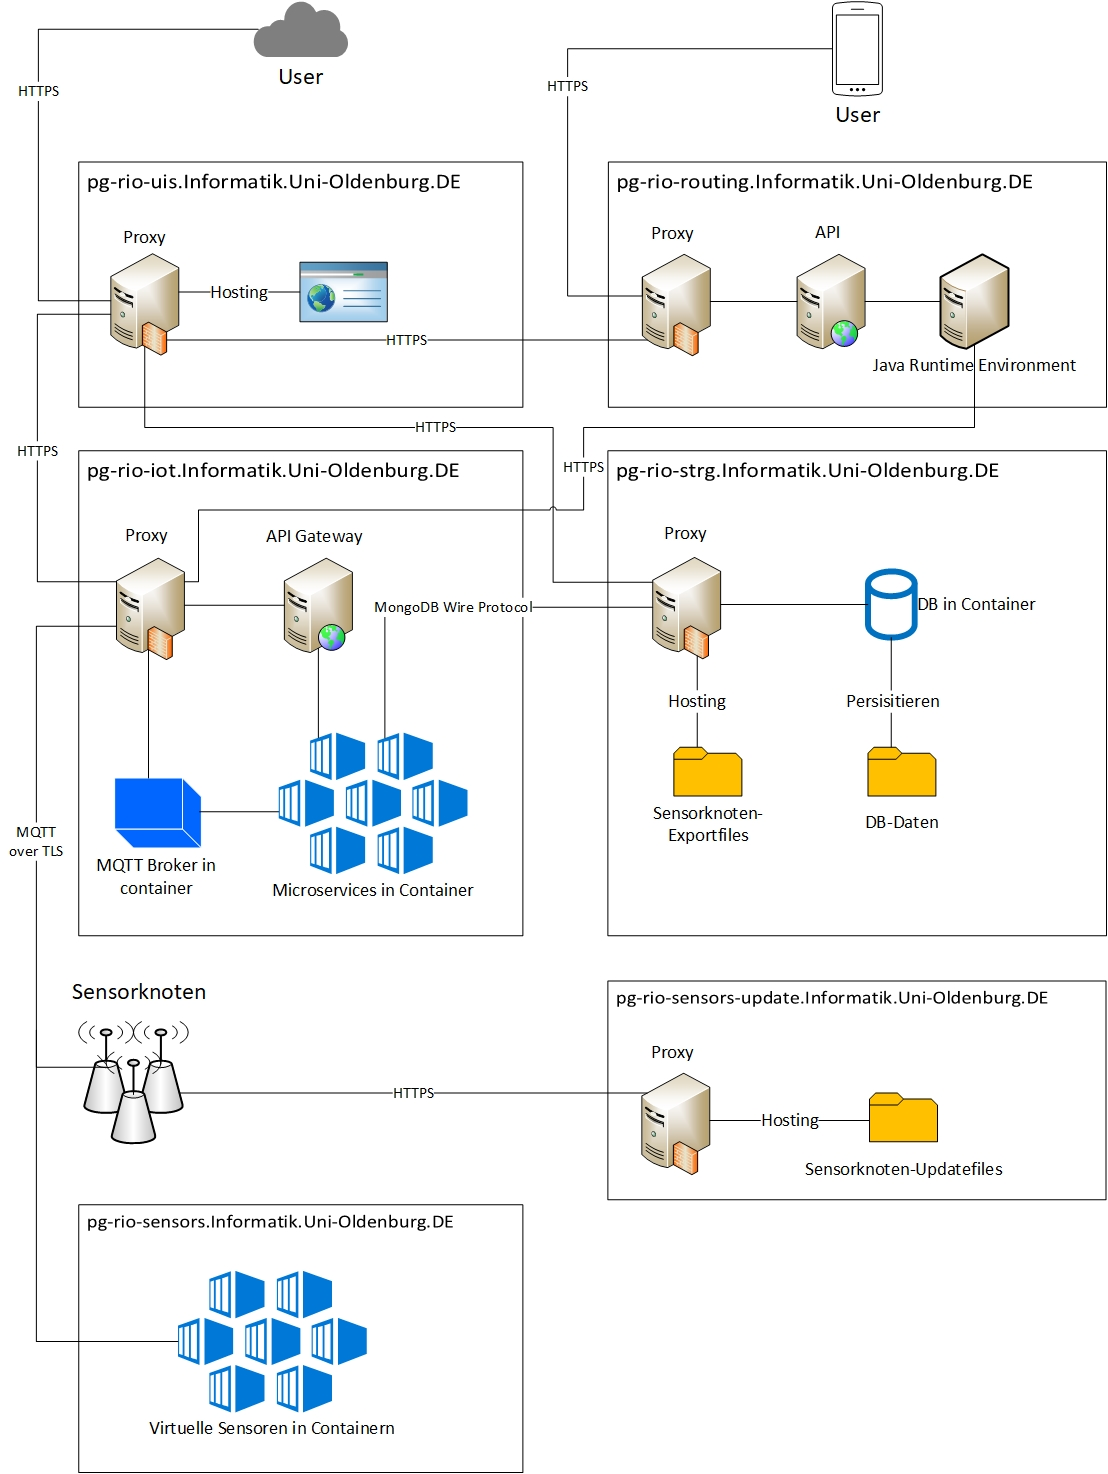
\includegraphics[scale=0.5]{ressourcen/Infrastruktur}
	\caption{Netzwerkdiagramm Infrastruktur}
	\label{fig:infrastruktur}
\end{figure}
\newpage

Alle Anfragen nach Diensten auf einer VM werden von einen Proxy-Server entgegengenommen und intern weitergeleitet.
Das ermöglicht die Abkapselung der Dienste innerhalb einer VM nach außen, die nicht direkt angesprochen werden sollen.
Bei allen Proxy-Servern kommt dazu der weit verbreitete Webserver NGINX (https://www.nginx.com/) zum Einsatz, der diese Funktionalität bietet.
Alle in \Fig{infrastruktur} dargestellten Server mit der Bezeichnung: Proxy, sind aktuelle Installationen des Webservers NGINX und für diesen Einsatzzweck konfiguriert.
Neben der Funktion des Proxy-Servers übernehmen die Server auch bei Erfordernis das Bereitstellen (Hosting) von: Webseiten, Exportdateien und Sensorknoten-Updatedateien.
Um verschlüsselte Kommunikation über die Proxy-Server zu ermöglichen, werden die frei erhältlichen Let's Encrypt Zertifikate (https://letsencrypt.org/de/) verwendet.
Zur Installation und Aktualisierung der Zertifikate wird das frei erhältliche Programm: certbot (https://certbot.eff.org/), verwendet.
In folgender Auflistung sind alle über die Proxy-Server erreichbaren Dienste, sowie alle Dienste innerhalb einer VM dargelegt:
in \Tbl{dieuis} die externen und VM internen Dienste der UIS-VM,
in \Tbl{dierouting} die externen und VM internen Dienste der Routing-VM,
in \Tbl{dieiot} die internen und VM internen Dienste der IoT-VM,
in \Tbl{diedb} die internen und VM internen Dienste der Datenbank-VM,
in \Tbl{vmsen} der interne Dienst der Sensorknoten-VM,
in \Tbl{vmsenup} der externe Dienst der Sensorknoten-Update-VM,
in \Tbl{vmbuild} der externe und VM interne Dienst der Build-Server-VM.\par\bigskip
\begin{table}[H]\caption{Dienste UIS-VM}\label{tbl:dieuis}
\begin{tabularx}{\textwidth}{|l|X|}
	\hline
	&  \textbf{pg-rio-uis.Informatik.Uni-Oldenburg.DE}\\ 
	\hline Proxy Extern
	& HTTPS Port 443:\\
	& - Entgegennahmen und Bearbeitung Service-Anfragen\\
	& - Redirect auf HTTPS Port 443 von HTTP Port 80\\
	& - Interne Weiterleitung auf HTTP Port 4200\\
	& - Stellt Anfragen an IoT-Plattform\\
	& - Stellt Anfragen an Routing zum Abrufen von Heatmaps\\
	& - Stellt Anfragen an DB-Server zum Abrufen von Sensorkonten-Exportfiles\\
	\hline VM Intern
	&  HTTP Port 4200:\\
	& - Hosting Webseite über internen Webserver\\	 
	\hline
\end{tabularx}
\end{table} 
\par\bigskip 

\begin{table}[H]\caption{Dienste Routing-VM}\label{tbl:dierouting}
\begin{tabularx}{\textwidth}{|l|X|}
	\hline
	&  \textbf{pg-rio-routing.Informatik.Uni-Oldenburg.DE}\\ 
	\hline Proxy Extern
	& HTTPS Port 9093:\\
	& - Interne Weiterleitung auf HTTP Port 9090\\
	\hline VM Intern
	&  HTTP Port 9090:\\
	& - Bereitstellung Routen\\
	& - Bereitstellung Heatmap\\	 
	\hline
\end{tabularx}
\end{table} 
\par\bigskip

\begin{table}[H]\caption{Dienste IoT-VM}\label{tbl:dieiot}
\begin{tabularx}{\textwidth}{|l|X|}
	\hline
	&  \textbf{pg-rio-iot.Informatik.Uni-Oldenburg.DE}\\ 
	\hline Proxy Intern
	& HTTPS Port 8443:\\
	& - Interne Weiterleitung auf HTTP Port 8080\\
	& MQTT over TLS Port 8883:\\
	& - Interne Weiterleitung auf MQTT Port 1883\\
	& MQTT over TLS (self"=signed) Port 8884:\\
	& - Interne Weiterleitung auf MQTT Port 1883\\ 
	\hline VM Intern
	&  HTTP Port 9090:\\
	& - Authentifizierungs-Dienst\\
	&MQTT Port 1883:\\
	& - MQTT-Broker\\	
	&HTTP Port 8080:\\
	& - Gateway\\	
	&HTTP Port 3000:\\
	& - PM25-Service\\	
	&HTTP Port 3004:\\
	& - Temperatur-Service\\	
	&HTTP Port 3002:\\
	& - Sensorknoten-Verwaltungs-Service\\	
	&HTTP Port 3001:\\
	& - Umweltinformationssystem-Service\\		 
	\hline
\end{tabularx}
\end{table} 
\par\bigskip 

\begin{table}[H]\caption{Dienste Datenbank-VM}\label{tbl:diedb}
\begin{tabularx}{\textwidth}{|l|X|}
	\hline
	&  \textbf{pg-rio-strg.Informatik.Uni-Oldenburg.DE}\\ 
	\hline Proxy Intern
	& HTTPS Port 443:\\
	& - Hosting Sensorknoten-Exportfiles\\
	& MongoDB Wire Protocol Port 27010, nur erlaubt von pg-rio-iot.Informatik.Uni-Oldenburg.DE:\\
	& - Interne Weiterleitung auf MongoDB Wire Protocol Port 27017\\
	\hline VM Intern
	&  MongoDB Wire Protocol Port 27017:\\
	& - MongoDB\\	 
	\hline
\end{tabularx}
\end{table} 
\par\bigskip 

\begin{table}[H]\caption{Dienste Sensorknoten-VM}\label{tbl:diesen}
\begin{tabularx}{\textwidth}{|l|X|}
	\hline
	&  \textbf{pg-rio-sensors.Informatik.Uni-Oldenburg.DE}\\ 
	\hline Intern
	& MQTT over TLS Port 8883:\\
	& - Virtuelle Sensorknoten\\	 
	\hline
\end{tabularx}
\end{table} 
\par\bigskip 

\begin{table}[H]\caption{Dienste Sensorknoten-Update-VM}\label{tbl:diesenup}
\begin{tabularx}{\textwidth}{|l|X|}
	\hline
	&  \textbf{pg-rio-sensors-update.Informatik.Uni-Oldenburg.DE}\\ 
	\hline Proxy Extern
	& HTTPS Port 443:\\
	& - Hosting Sensorknoten-Updatefiles\\
	& HTTPS (self"=signed) Port 444:\\
	& - Hosting Sensorknoten-Updatefiles\\	 
	\hline
\end{tabularx}
\end{table}
\par\bigskip

Zur Unterstützung von CI/CD-Prozessen wird die frei erhältliche CI/CD-Software Jenkins Blue Ocean eingesetzt (https://jenkins.io/projects/blueocean/). Dazu werden folgende Dienste bereitgestellt:\par\bigskip
\begin{table}[H]\caption{Dienste Build-Server-VM}\label{tbl:diebuild}
\begin{tabularx}{\textwidth}{|l|X|}
	\hline
	&  \textbf{pg-rio-build.Informatik.Uni-Oldenburg.DE}\\ 
	\hline Proxy Extern
	& HTTPS Port 443:\\
	& - Interne Weiterleitung auf HTTP Port 8080\\
	\hline VM Intern
	&  HTTP Port 8080:\\
	& - Jenkins-Verwaltungsoberfläche (Anmeldung erforderlich)\\	 
	\hline
\end{tabularx}
\end{table} 
\par\bigskip 

